\chapter{Introducción}
La luz es la parte de espectro electromagnético que puede ser percibida por el
ojo humano, esta tiene impacto sobre la vida sin importar de que fuente
provenga. A finales del siglo XIX y principios del siglo XX se dieron avances
científicos y tecnológicos en la óptica que dieron paso al desarrollo tecnológico
de fuentes artificiales entre las que incluyen, la bombilla incandescente,
seguido de otras fuentes de iluminación como, las lámparas fluorescentes,
halógenas, los diodos Emisores de Luz y recientemente los LED orgánicos\cite{Sustentable2014}.
Cada una de estas tecnologías de iluminación ha
experimentado un cambio constante debido a mejoras en los materiales,
diseño, calidad de luz, eficiencia energética y la eficiencia en el proceso de
fabricación. Desde sus inicios hasta la actualidad, la iluminación de estado
sólido ha sido líder en la industria de la iluminación, en donde,
los dispositivos más conocidos y ampliamente empleados son los LED combinados
con fósforos\cite{ISR-UniversidaddeCoimbra2017,Bernal2016}.\\

En la actualidad no existe ningún LED capaz de generar directamente luz blanca. 
En el diodo emisor de luz blanca (wLED), se obtiene mediante la mezcla de
varios colores, que
se obtiene de la combinación de emisión de luz azul y un fósforo amarillo,
sin embargo, los wLED no pueden alcanzar potencias altas de manera nativa,
debido a que, la naturaleza del funcionamiento de estos dispositivos
les impide mantener
su eficiencia a altas densidades de corriente eléctrica. Los diodos
láser (LD) pueden alcanzar potencias elevadas sin perder eficiencia, pero esto
conlleva a otra dificultad y es la degradación del fósforo. Por lo tanto,
se suele incorporar los fósforos en resinas orgánicas, pero estos
materiales no son capaces de resistir la potencia de un LD. Por lo tanto, es
necesario emplear materiales más resistentes, por ejemplo, los materiales
cerámicos que presentan una mejor conductividad térmica y estabilidad química a
temperaturas mayores que las resinas\cite{AlvarezJauregui2020}, permitiendo que los diodos
emisores de luz tengan aplicaciones tanto para baja potencia como alta
potencia, por lo que se usan con gran frecuencia en la industria de comunicación,
alimentos y
salud. En todas estas aplicaciones, la potencia óptica requerida puede llegar a
variar desde menos de un Watt hasta centenas de Watts. La eficiencia de los
LEDs, solo se presenta cuando trabajan a bajas densidades de potencia, esto se
debe al fenómeno conocido como “Caída térmica”, que se evalúa en LEDs
de InGaN de alta calidad, para determinar si sus fallas son
causadas por variaciones intrínsecas en la recombinación o por efectos de
transporte\cite{Baur2018}.\\

Existen diferentes tipos de procesos para la fabricación de wLEDs, que se basan 
en la conversión de longitud de onda o la mezclas de LEDs de diferente color. El
método de conversión de longitud de onda se basa en mezclar un componente de longitud 
de onda larga con un componente de longitud de onda más corta, en donde se han empleado 
combinaciones de LED azul o UV con fósforos amarillos y mezclas de fósforos verdes
y rojos. Los fósforos de aluminato llaman la atención debido a su eficiencia de
conversión cuántica, buena reproducción cromática y amplio rango de excitación.
Los fósforos de aluminato más conocidos son \ce{Y_{3}Al_{5}O_{12}}:\ce{Ce^{3+}} y sus
variaciones. El primer pc-wLED se fabricó combinando el fósforo de granate de itrio
aluminio dopado con cerio \ce{Y_{3}Al_{5}O_{12}}:\ce{Ce^{3+}} (YAG:\ce{Ce^{3+}}) 
de color amarillo 
con un chip de \ce{InGaN} emisor de luz azul, mediante una mezcla equilibrada
de estos componentes se logra producir la apariencia de luz blanca, sin embargo,
la luz resultante tiene ausencia del componente rojo, de tal manera que su
temperatura de color es alta y presenta un indice de reproducción cromática 
(CRI) bajo\cite{Sustentable2014,Li2005,khanna2014}.\\

Los fósforos utilizados en los wLED tienen un papel importante en la
determinación de la calidad de la luz blanca, estos consisten en una matriz y
un activador. Para obtener una fuente de luz de estado sólido de alta calidad,
los fósforos utilizados en LED deben presentar características básicas como: el
espectro de excitación, que combina los chips LED que muestran una gran
intensidad de absorción de luz azul. Existen métodos para diseñar y desarrollar
los fósforos LED, que incluyen la investigación y evaluación de diferentes
fósforos anfitriones para wLED  (tales como granates, (oxo) nitruro,
aluminato, borato, silicato, sulfuros, fosfatos etc.)\cite{Li2005}.\\

Los dispositivos en su mayoría los pc-wLEDs se basan en YAG:\ce{Ce^{3+}}, 
como material
de luminiscencia que emite luz amarilla, en varios estudios se ha usado
al YAG:\ce{Ce^{3+}} y sus modificaciones de composición bajo la siguiente ecuación
\ce{(Y,Gd)_{3}(Al,Ga)_{5}O_{12}}:\ce{Ce^{3+}}, sustituyendo átomos con la finalidad
de alterar el comportamiento y determinar las características de funcionamiento. 
Los fósforos dopados con \ce{Ce^{3+}} siguen siendo los más óptimos para la 
fabricación de
dispositivos LED comerciales debido a que se obtiene una combinación de alta
eficiencia luminosa y excelente rendimiento, por lo tanto, se puede inferir que 
los fósforos dopados con \ce{Ce^{3+}} permiten ajustar las propiedades de 
luminiscencia y emisión, lo que facilita adaptarse a diferentes aplicaciones\cite{Ahn2017}.\\

La familia de compuestos de silicato juegan un papel importante en el diseño de 
nuevos fósforos, especialmente los silicatos que cristalizan en forma ortorrómbica,
\ce{(A,B)_{2}SiO_{4}} A,B= \ce{Ca, Sr, Ba}, han recibido interés debido a su uso
potencial como unidades estructurales básicas los silicatos [\ce{SiO_{4}}] 
pueden constituir estructuras cristalinas
complejas, que contienen una amplia variedad de grupos aniónicos, a través de
diferentes métodos de conexión. Entre estas, las fases \ce{(A, B)_{2}SiO_{4}},
\ce{A_{3}SiO_{5}}, \ce{Li_{2}ASiO_{4}} y \ce{Ca_{3}Sc_{2}Si_{3}O_{12}} 
son las más comunes y sus propiedades de luminiscencia permiten su aplicación en fabricación de LED. 
Los silicatos activados con tierras raras se utilizan ampliamente como fósforos
wLED estos tienen composiciones químicas y estructuras cristalinas versátiles,
propiedades de luminiscencia ajustables, algunos de los fósforos de silicato
sintetizados son \ce{Ca_{3}Sc_{2}Si_{3}O_{12}}, \ce{A_{3}B_{2}C_{3}O_{12}}, 
\ce{M_{5}(Si_{3}O_{9})_{2}} y \ce{Ca_{3}Si_{2}O_{7}}\cite{Wu2018}.\\


Actualmente, se encuentra el fósforo de fluoruro activado por \ce{Mn^{4+}}, 
como \ce{K_{2}SiF_{6}}:\ce{Mn^{4+}} y
\ce{BaSiF_{6}}:\ce{Mn^{4+}}, que se usan para mejorar la reproducción del color
para wLED. El fósforo de \ce{Mn^{4+}} puede absorber la
luz azul y mostrar una emisión roja de tipo línea originada en la transición d-d
de \ce{Mn^{4+}}. Los fósforos de floruro dopados con \ce{Mn^{4+}} han sido 
ampliamente estudiados, centrándose en los nuevos tipos estructurales, diferentes
métodos de síntesis, la evaluación y aplicación en dispositivos wLED. Sin embargo,
el principal problema es que este tipo de sistemas es que generalmente se preparan
mediante el método basado en solución, que consume mucha agua, solución de fluoruro
de hidrógeno (HF) y oxidante, lo que genera una alta probabilidad de contaminación 
en etapas posteriores de fabricación en masa. Además, el ión Mn es muy sensible 
a diferentes condiciones de reacción y puede existir en múltiples estados de valencia,
incluidos \ce{Mn^{2+}}, \ce{Mn^{3+}}, \ce{Mn^{4+}}, \ce{Mn^{6+}} y \ce{Mn^{7+}}, 
por lo que se debe controlar las condiciones de síntesis adecuadas, de lo contrario 
afectará la calidad del fósforo obtenido\cite{Wu2018}.\\

Se han reportado muchos materiales de fosfato prometedores, entre ellos, los
fósforos de cloropatita \ce{Ca_{5}(PO_{4})_{3}Cl}:\ce{Eu^{2+}} de tipo
apatito que tienen una larga historia de uso en la industria de iluminación y
exhibición, sin embargo, la absorción óptima de estos fósforos dopados con
\ce{Eu} rara vez coincide con la emisión de LEDs azules, es decir, la mayoría de
estos solo podrían producirse con chips LED n-UV en el rango de longitud de
onda 350-420 nm. Los boratos también juegan un papel importante en la familia
de materiales luminiscentes y han atraído mucha atención debido a su
estabilidad, potencial síntesis de bajo costo y características que los hacen
amigables con el medio ambiente, por ejemplo, se conoce la sinterización de
\ce{LiSr_{4}(BO_{3})_{3}}, \ce{NaSr_{4}(BO_{3})_{3}}, \ce{NaSrBO_{3}}, \ce{Na_{3}SrB_{5}O_{10}},
\ce{NaSrB_{5}O_{9}} y \ce{NaBa_{4}(BO_{3})_{3}}\cite{Wu2018}.\\

El fósforo rojo \ce{Li_{2}MgGeO_{4}}:\ce{Mn^{4+}} se sintetizó mediante un método de
estado sólido a alta temperatura en aire. La banda de fotoluminiscencia
más fuerte se presenta a 671 nm en el rango de (600-750) nm, este proceso se debe
a la transición \ce{^{2}E -> ^{4}A_{2}} del ión \ce{Mn^{4+}} y los espectros PLE
(fotoluminiscencia de excitación) muestran un pico de banda ancha en 323 nm dentro
del rango 220-550 nm debido a las transiciones \ce{^{4}A_{2} ->^{4}T_{1}} del ión
Mn\cite{Cao2015}. Los fósforos rojos comerciales, como los nitruros activados
con \ce{Eu^{2+}}, oxinitruros, sulfuros y fluoruros activados con \ce{Mn^{4+}}
tienen dificultad para ser introducidos en la matriz de vidrio para obtener el
rojo YAG:\ce{Ce^{3+}} + PiG (PiG = fósforo en vidrio). Además, tal distribución aleatoria de los
fósforos en la matriz de vidrio da como resultado la reabsorción de fotones y
reducirá la eficiencia de emisión\cite{Chen2016}. Una estrategia alternativa
para resolver esos problemas es la exploración de configuración geométrica para
lograr una emisión de banda ancha y altamente eficiente de wLED, Lee et al. y Ying 2016
desarrollaron una nuevo diseño de configuración para disminuir la superposición
espectral cortando y volviendo a ensamblar para obtener 2 piezas (2-PiG) y 
4 piezas (4-PiG), LuAG:\ce{Ce^{3+}} + PiG y \ce{CaAlSiN_{3}}:\ce{Eu^{2+}} +
PiG. Donde, se observa el apilamiento de capa de fósforo rojo con recubrimiento
en YAG:\ce{Ce^{3+}} + PiG para obtener una emisión blanca cálida 
con una alta eficiencia luminosa, Chen et al. desarrollaron la misma configuración de
apilamiento por acoplamiento secuencial de YAG:\ce{Ce^{3+}} + PiG y
YAG:\ce{Mn^{4+}}/\ce{Mn^{2+}} + PiG con un chip azul InGaN para producir blanco
cálido de esta manera se puede dar a conocer los diferentes tipos de síntesis
con dopaje con \ce{Mn^{4+}} y su función a la producción de
LEDs\cite{Lin2015,Xiang2016}.\\


Los fósforos dopados con \ce{Eu^{2+}} y \ce{Ce^{3+}} se convierten en los
materiales dopantes más sobresalientes en el campo la fabricación de fósforos
para wLED. Los fósforos rojos dopados con \ce{Eu^{3+}} son otra serie de
importantes sistemas de fósforo, especialmente los fósforos rojos
basados en tungstatos/molibdatos. En los tungstatos o molibdatos sustituidos
con \ce{Eu^{3+}} y sus soluciones sólidas, el espectro contiene una amplia
banda de absorción que va desde (250 a 400) nm y esta banda se atribuye a la
transición de oxígeno a tungsteno/molibdeno\cite{Kasturi2016,Wu2018}.\\

Los granates de lutecio aluminio (LuAG) se han sintetizado por
diferentes métodos, sin embargo, existen falencias como la elevada temperatura
requerida en el proceso (más de 1400$^{\circ}$C) o la necesidad de equipos costosos y
sofisticados. Por otro lado, el LuAG no cuenta con propiedades magnéticas como
el YIG, limitando su campo de aplicación. El trabajo de investigación realizado
permitió conocer el efecto de sustituir cationes \ce{Al^{3+}} por cationes \ce{Fe^{3+}} sobre
las propiedades estructurales, magnéticas y ópticas del granate
\ce{Ce^{3+}}:\ce{Lu_{3}Al_{5}O_{12}}.\\

Los granates naturales y sintéticos forman una familia de materiales que
se relacionan en su estructura y propiedades físicas, lo que genera su
aplicabilidad, principalmente en los ámbitos eléctrico, magnético y óptico.
Estas propiedades son influenciadas principalmente por su composición química
como por las modificaciones estructurales, generadas a través de sustituciones
isomórficas en la red cristalina\cite{Chenais2003}. La versatilidad en la
composición y los métodos empleados para su obtención, convierten a los
granates en materiales útiles en una gran variedad de aplicaciones en
dispositivos de última generación. Entre los materiales tipo granate se
destacan los constituidos por elementos de tierras raras, estos presentan
caracterizas prominentes como una alta estabilidad térmica, elevada dureza,
isotropía óptica y alta conductividad térmica\cite{MartinPereda1976,Mari2001,Liu2014,Birkel2012,Heer2002,Malinowski1999}.\\

Algunos ejemplos relevantes de granates derivados de elementos de tierras
raras, son el granate hierro-lutecio (\ce{Lu_{3}Fe_{5}O_{12}}), el cual presenta
propiedades magnéticas que permiten su aplicación en dispositivos aisladores de
microondas, circuladores, rotadores de Faraday y filtros de onda\cite{Basavad2020,Crisp1998,Neel1964},
 lo que ha conllevado a un amplio estudio
y aplicabilidad, por otro lado el granate de aluminio-lutecio dopado con cerio
(\ce{Ce^{3+}}:\ce{Lu_{3}Al_{5}O_{12}}), presenta propiedades ópticas que permiten su
potencial aplicación en una amplia variedad de dispositivos emisores de luz,
como una red de acogida para medios de ganancia en láseres de estado sólido,
cristales de centelleo y materiales luminiscentes para lámparas de descarga y
dispositivos LED\cite{Ionov2005,Mares2004,Tous2008,Pan2004,Katelnikovas2008}.
Pese a las múltiples aplicaciones potenciales, estos materiales se encuentran
restringidos en su campo de acción, por presentar solo un tipo de propiedad.
Una característica adicional y muy importante que presentan los granates que
contienen lutecio, es el denominado fenómeno de “corte cuántico”, proceso por
en el cual un fotón de alta energía se transforma en dos fotones de menor
energía\cite{Yarici2016}. El proceso de corte cuántico es de particular
interés al poder convertir una radiación de longitud de onda corta tipo
ultravioleta visible (UV-vis) en dos o más emisiones de infrarrojo cercano
(NIR), un proceso de gran importancia para mejorar la eficiencia de conversión
de las celdas solares de silicio las cuales presentan una baja eficiencia en la
región del ultravioleta visible\cite{Krsmanovic2007}.\\

En últimos años el desarrollo de diodos emisores de luz blanca (w-LED) ha
proporcionado un recurso importante para reducir el gasto energético a través
de la sustitución de las fuentes de iluminación convencionales\cite{Garskaite2007}, 
en este sentido, el método más común para crear la luz
blanca es la conversión parcial de la luz azul emitida por el granate de
aluminio-lutecio dopado con cerio (\ce{Ce^{3+}}:\ce{Lu_{3}Al_{5}O_{12}})\cite{Yamazaki1994}.
Si bien, la conversión de la luz azul es una ruta de generación de luz blanca,
económica y eficiente, se han demostrado los potenciales daños de la emisión
residual azul para la salud visual\cite{Psuja2007}, así como, la deficiente
reproducción de color debido a la deficiencia del componente rojo, lo cual
limita su aplicación en iluminación doméstica, adicional a ello el lutecio
carece de propiedades magnéticas aprovechables, por lo cual le ha visto
rezagado frente a investigaciones de los granates le aluminio-itrio
(\ce{Y3Al5O12}), que debido a su versatilidad magneto-óptica, es apto para
aplicaciones de alta frecuencia, microondas, circuladores, aisladores y
dispositivos de cambio de fase\cite{Hapishah2017,Setlur2006}.\\

Chenyao Zhao y Yotong Duan en el año 2020, realizaron estudios de síntesis y
caracterización de propiedades de cerámicas en donde se tiene como componente
el LuaG, en este estudio se preparan cerámicas transparentes mediante una
reacción de estado sólido a alta temperatura en una atmósfera de \ce{O_{2}}. De acuerdo
con los espectros PL y las curvas de disminución de la emisión, la energía se
transfirió de \ce{Ce^{3+}} a \ce{Mn^{2+}} a través de una transición no
radiactiva. Mediante el control de la concentración de
\ce{Mn^{2+}}-\ce{Si^{4+}} iones, la luz emitida cambió de verde a naranja. Por
lo tanto, las cerámicas transparentes LuAG co-dopadas con \ce{Ce} y \ce{Mn} de color
ajustable son adecuadas para aplicación en la fabricación de los LED blancos\cite{Zhao2021}. 
Este tipo de estudio se puede comparar con el de Bing Yan, Yi
Wei,  donde proporciona una visión para lograr una modulación de emisión de
rojo, sin embargo, la modulación de la posición de pico espectral y el ancho de
banda siguen siendo desafíos cruciales. Se diseño la transferencia de energía
\ce{Eu^{3+}} → \ce{Mn^{4+}} en el anfitrión de granate \ce{Lu3Al5O12} (LuAG).
Por otro lado, LuAG:\ce{Eu^{3+}} exhibe propiedades anti-templado térmico, es
decir, la intensidad máxima alcanza el 166\% a 200$^{\circ}$C de la intensidad inicial a
25$^{\circ}$C. La transferencia de energía de \ce{Eu^{3+}} → \ce{Mn^{4+}}, el
rendimiento de enfriamiento térmico de \ce{Mn^{4+}} se mejora drásticamente.
Las intensidades de pico de fotoluminiscencia a 668 nm para
LuAG:0.01\ce{Mn^{4+}} y LuAG: 0.05 \ce{Eu^{3+}}, 0.01\ce{Mn^{4+}} retienen
3.26\% y 26\% a 200$^{\circ}$C de la intensidad original a 25$^{\circ}$C \cite{Yan2021}.\\

En el año 2018 el autor Florián Baur y Thomas, ponen en marcha un proyecto
donde los fósforos emisores de rojo de banda estrecha tienen un gran potencial
para aumentar la eficacia luminosa de los LED de color blanco cálido si su
espectro de emisión alcanza un pico entre 610 y 630 nm y la reabsorción de la
luz emitida por el fósforo LED verde a amarillo, ejemplo LuAG:Ce o YAG:Ce. El
polvo se calcino a 1000$^{\circ}$C durante 4 horas en aire, este polvo resultante mostró
un color amarillo ligeramente verdoso, donde la decoloración es probablemente
el resultado de la formación de \ce{U^{5+}}, la mezcla se sintetizo varias
veces a 1100$^{\circ}$C o en \ce{O2} hasta conseguir un cambio de color a amarillo
claro, el mineral se trituro en un molino hasta convertirlo un fino polvo negro
y se dispersó en una solución 10:1 de 90\% de \ce{H2SO4}  y 30\% de \ce{H2O2} ,
la mezcla se mantuvo a 90$^{\circ}$C con agitación durante 3 días, la eficiencia
cuántica definida como la relación entre los fotones absorbidos y el número de
fotones emitidos se determinó en un 78\% con una excitación de 410 nm. Los
materiales de tipo fluoruro dopado con \ce{Mn^{4+}} dominan la búsqueda de
tales fósforos novedosos. En este trabajo observa la sensibilización de la
fotoluminiscencia de \ce{Eu^{3+}} por cationes de uranilo en
\ce{K4(UO2)Eu2(Ge2O7)}. al obtener estos resultados de enfoque que produce un
fósforo con una eficacia luminosa de 260 lm W$_{opt}$ $^{-1}$ con un punto de
color CIE 1931 de x = 0.647 e y = 0.349 la simulación de los espectros de los
LED y de un LED blanco cálido preparado a partir de un LED de 465 nm con una
cúpula compuesta por YAG:Ce y \ce{K4(UO2)Eu2(Ge2O7)} revela que el pcLED blanco
muestra una eficiencia lumínica  de 360 lm W$_{opt}$ $^{-1}$, la simulación de
espectros LED basado en un LED de 465 nm con una cúpula de silicio que
comprende YAG:Ce y \ce{K4(UO2)Eu2(Ge2O7)2} revela que el pcLED blanco cálido
muestra una eficacia luminosa ultra alta de 360 lm W$_{opt}$ $^{-1}$
mientras se mantiene un CRI alto, estos resultados subrayan que el catión
uranilo es un sensibilizador adecuado para los fósforos LED emisores de rojo
activados por el activador muy eficiente y estable
\ce{Eu^{3+}}\cite{Baur2018,LiuFlux}.\\

El autor Run Xiang y sus colaboradores en el año 2016 sintetizaron material
mediante dos pasos principales, un nuevo LuAG:\ce{Ce^{3+}} fósforo en vidrio
(Lu-PiG) que se combina con la capa de fósforo rojo \ce{CaAlSiN3}:\ce{Eu^{2+}}
se sintetizó mediante las técnicas de co-sinterización a baja temperatura y
serigrafía, que se demostró experimentalmente para reemplazar el convertidor de
fósforo convencional basado en polímeros y se realizó el ajuste de cromaticidad
para el fósforo LuAG:\ce{Ce^{3+}}. Las placas de Lu-PiG se prepararon mediante
la técnica de co-sinterización a una baja temperatura, en este proceso incluían
los fósforos comerciales LuAG:\ce{Ce^{3+}} \cite{Han2019,Peng2020}.\\

Shangjun yu y QI Chen en el año 2020  nos introduce en la aparición del led
blanco (YAG:\ce{Ce^{3+}}) este se ha convertido en uno de los fósforos más
usados en la fabricación de LEDs, aun así se evidencian contaminación baja  en
la síntesis de este material, el presente articulo  realizan un procedimiento
donde se caracteriza patrones de materiales para sinterizar una nueva luz Led,
los materiales usados tienen óxidos de tierras raras, monóxido de manganeso,
oxido de aluminio, sílice, alcohol,  estos tipos de reactivos se usan sin
necesidad de ser purificados,  los materiales propuestos se prepararon por el
método  de fase solida a alta temperatura, los elementos restantes se colocaron
en un depósito de molienda en constante agitación por 10 horas para garantizar
la mezcla de materiales, se secó la mezcla 80 grados centígrados durante 245
horas para obtener el precursor se molió y paso por un tamiz de 200 mallas, se
calcino  a  1.500$^{\circ}$C durante 4 horas, por consiguiente de caracterizo, esto
patrones se obtuvieron a temperatura ambiente usando la radiación, la
morfología de precursor y de los productos restantes  fueron recogidos, los
rendimiento ópticos de  las muestras se realizaron  en condiciones idénticas,
entre los resultados del estudio podemos apreciar que el fósforo sigue siendo
la fase pura como dosis de \ce{Mn^{2+}}/\ce{Si^{4+}}, el fósforo sigue siendo
la estructura del granate de aluminio y gadolinio cuando se calcina a 1.500$^{\circ}$C
lo que indica que el dopaje  de \ce{Y^{3+}} es eficaz para estabilizar  la
estructura de granate\cite{Yu2021}.\\

En la fabricación de fósforo  a partir de granate, Big Yan y
Yin Wei en el 2020  menciona  el trabajo realizado con fósforo de granate LuAG
ajustable en rojo mediante transferencia de energía \ce{Eu^{3+}} -
\ce{Mn^{4+}} y su uso para  en la aplicación de sensores ópticos de
termometría, los fósforos emisores de rojo desempeñan en la iluminación, pico
de emisión óptimo se sitúa en (620-630) nm, midiendo este factor se puede deducir
que posee alto rendimiento cuántico de luminiscencia, estabilidad térmica,
forma e intensidad espectral, de la misma manera estabilidad física, estos
fósforos  pueden tener aplicaciones  potenciales de sensores ópticos, este
diseño de  la transferencia  de energía \ce{Eu^{3+}}-\ce{Mn^{4+}} pude lograr
una emisión  de color desde el rojo al naranja, los resultados obtenidos en el
estudio nos dicen que el \ce{Lu3AI5O12} es conocido como un tipo de granate
típico con una estructura altamente simétrica y rígida, dando como resultado
factores de fiabilidad aceptables, indicando la incorporación de \ce{Eu^{3+}} y
\ce{Mn^{4+}} no influye en la estructura cristalina del huésped LuAG,
realizando la síntesis de este tipo de mineral se pueden observar en el estudio
que  se ha conseguido un fósforo  de granate LuAG:\ce{Eu^{3+}}, \ce{Mn^{4+}}
ajustable mediante el diseño de la transferencia de energía \ce{Eu^{3+}}
\ce{Mn^{4+}} siendo esta en particular  una transferencia de energía positiva
para la mejora del apagado térmico de \ce{Mn^{4+}}, dando a conocer la
sensibilidad de la temperatura que indica los fósforos LuAG:\ce{Eu^{3+}},
\ce{Mn^{4+}} teniendo potencial en sensores ópticos  de
termometría\cite{Yan2021}.\\

Los materiales multiferroicos magnetoeléctricos (MD) son compuestos que
muestran la coexistencia de ordenes eléctricos y magnéticos, y una variedad de
fenómenos de acoplo entre la polarización y la magnetización, estas propiedades
permitirían la aparición de nuevas tecnologías, tales como dispositivos
espintrónicos ajustables con un campo eléctrico, sensores magnéticos sin
enfriamiento, y memorias magneto-eléctricas, por lo tanto este tipo de
materiales han atraído mucho interés recientemente debido a la coexistencia de
órdenes ferro-eléctrico, ferromagnético y ferro-elástico. La posibilidad de
ajustar la permitividad dieléctrica por un campo magnético externo abre nuevas
perspectivas para la comprensión básica de materiales multiferroicos y para el
diseño de dispositivos basados en ellos. Pero el campo magnético requerido para
producir este efecto es bastante alto, en el orden de varios teslas. Sin
embargo, para la utilización de este efecto en los dispositivos antes
mencionados, se requiere de materiales que exhiban un efecto MD a campos
magnéticos bajos ($<$1T). Obtener el efecto MD con un pequeño campo magnético
externo no es común y tales materiales MD son todavía raros. Los granates de
hierro de tierras raras (RIG) con sus propiedades sorprendentemente
interesantes atraen una atención significativa. Se encontró que los materiales
que pertenecen a esta clase exhiben un efecto magneto-dieléctrico relativamente
bueno incluso para un bajo campo magnético aplicado. En campos magnéticos
bajos, se han informado efectos MD inducidos con valores que alcanzan el 13\% a
0.5 T y 10 K en \ce{Y3Fe5O12} y 3\% para H$<$0.2T por debajo de 30 K en
\ce{Tb3Fe5O12}\cite{Manimuthu2015}. Sin embargo, la mayoría de las aplicaciones
prácticas exigen un efecto MD a temperatura ambiente.\\

El \ce{Lu3Fe5O12} es uno de los compuestos que exhiben una respuesta MD a un
campo bajo a temperatura ambiente, pertenece a la familia RIG, tiene simetría
cúbica con el grupo espacial Ia(3d). La celda unitaria de \ce{Lu3Fe5O12} está
compuesta por grupos de lutecio-oxígeno y hierro-oxígeno que forman tres sitios
dodecaédricos (\ce{LuO8}), tres tetraédricos (\ce{FeO4}) y dos octaédricos
(\ce{FeO6}). Los iones \ce{Fe^{3+}} ocupan la posición Wyckoff 16a en el sitio
octaédrico (0 0 0) y la posición Wyckoff 24d en el sitio tetraédrico (0.375 0
0.25). Los iones \ce{Fe^{3+}} en los sitios octaédricos y tetraédricos se
denominan \ce{Fe^{1o}} y \ce{Fe^{2t}}, respectivamente. Los iones Lu se
distribuyen sobre la posición de Wyckoff 24c (0.125 0 0.25) en el sitio
dodecaédrico y el O está en el sitio de 96 h (-0.0255 0.0592 0.1514). Los iones
Fe en los sitios tetraédricos y octaédricos contribuyen a las propiedades
magnéticas que se acoplan de forma anti-paralela entre sí. El Lu en el sitio
dodecaédrico no posee momento magnético debido a la ausencia de electrones
desapareados ya que Lu tiene una configuración \ce{4f^14}. En general, el
material se reconoce y se evidencia como un material MD monofásico y, por lo
tanto, debe tener una anomalía dieléctrica a la temperatura de ordenamiento
magnético (independientemente del tipo de ordenamiento
magnético)\cite{Manimuthu2014}.

%%\ref{fig:luig}.
\begin{figure}[h]
    \centering%
    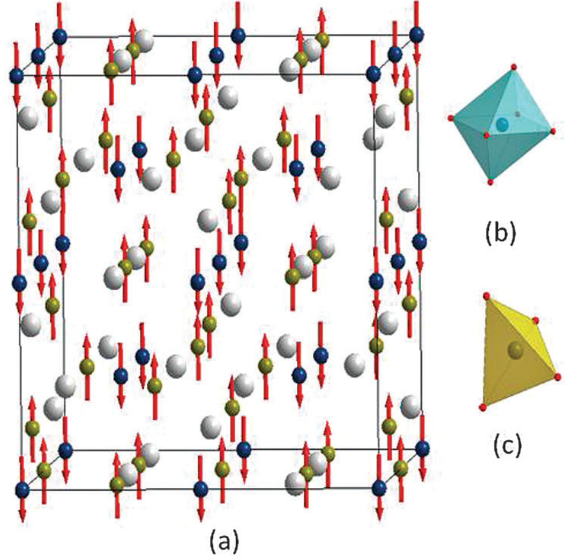
\includegraphics[scale=0.5]{Kap1/LuIG}%
    \caption{(a) Estructura magnética del \ce{Lu3Fe5O12}. Vista de (b) Octaedro
        y (c) tetraedro} \label{fig:luig}
\end{figure}






